\chapter{Anexo referente às imagens dos gráficos utilizados no relatório (TripAdvisor-Hóteis)}
\label{an1}

Uma vez que as imagens que retratam os gráficos elaborados são muito extensas, serão apenas mostradas algumas delas e em, cada secção apontado o link que redirecciona para o GitHub do projecto onde será possível aceder a cada imagem respectivamente assim como ao ficheiro \textit{.pbix} que contém os gráficos realizados no \textit{PowerBI}.
Inicialmente serão expostos os gráficos totais, anteriormente mostrados no \hyperref[cap7]{ capítulo 7 (Geração de gráficos)} exclusivamente para o \textit{website TripAdvisor} e acerca dos hotéis.

Acesso a todos os gráficos originados: \href{https://github.com/CatKinKitKat/pi2021/tree/master/projecto/datascience/graphs/TripAdvisor/hotels}{GitHub}.

\begin{figure}[!htb]
\centering
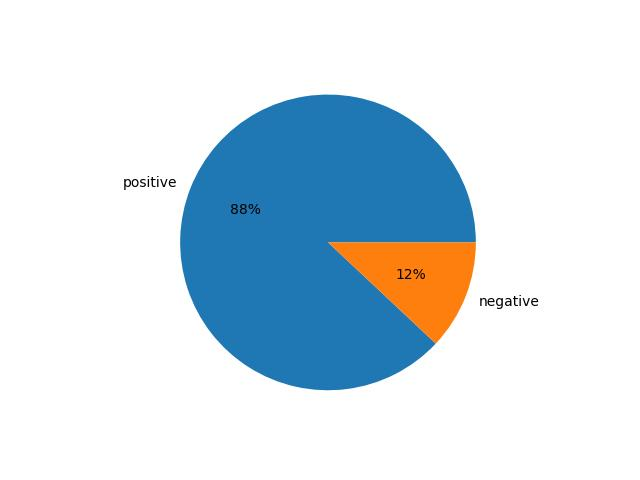
\includegraphics[width=7cm]{figuras/TripAdvisor/Hotels/hotel0_sentiments.jpeg}
\caption{Gráfico circular gerado baseando-se nos \textit{sentiments} mais usados da plataforma \textit{TripAdvisor} referente à Pousada Convento Beja}
\label{fig:exemplofig}
\end{figure}

\begin{figure}[!htb]
\centering
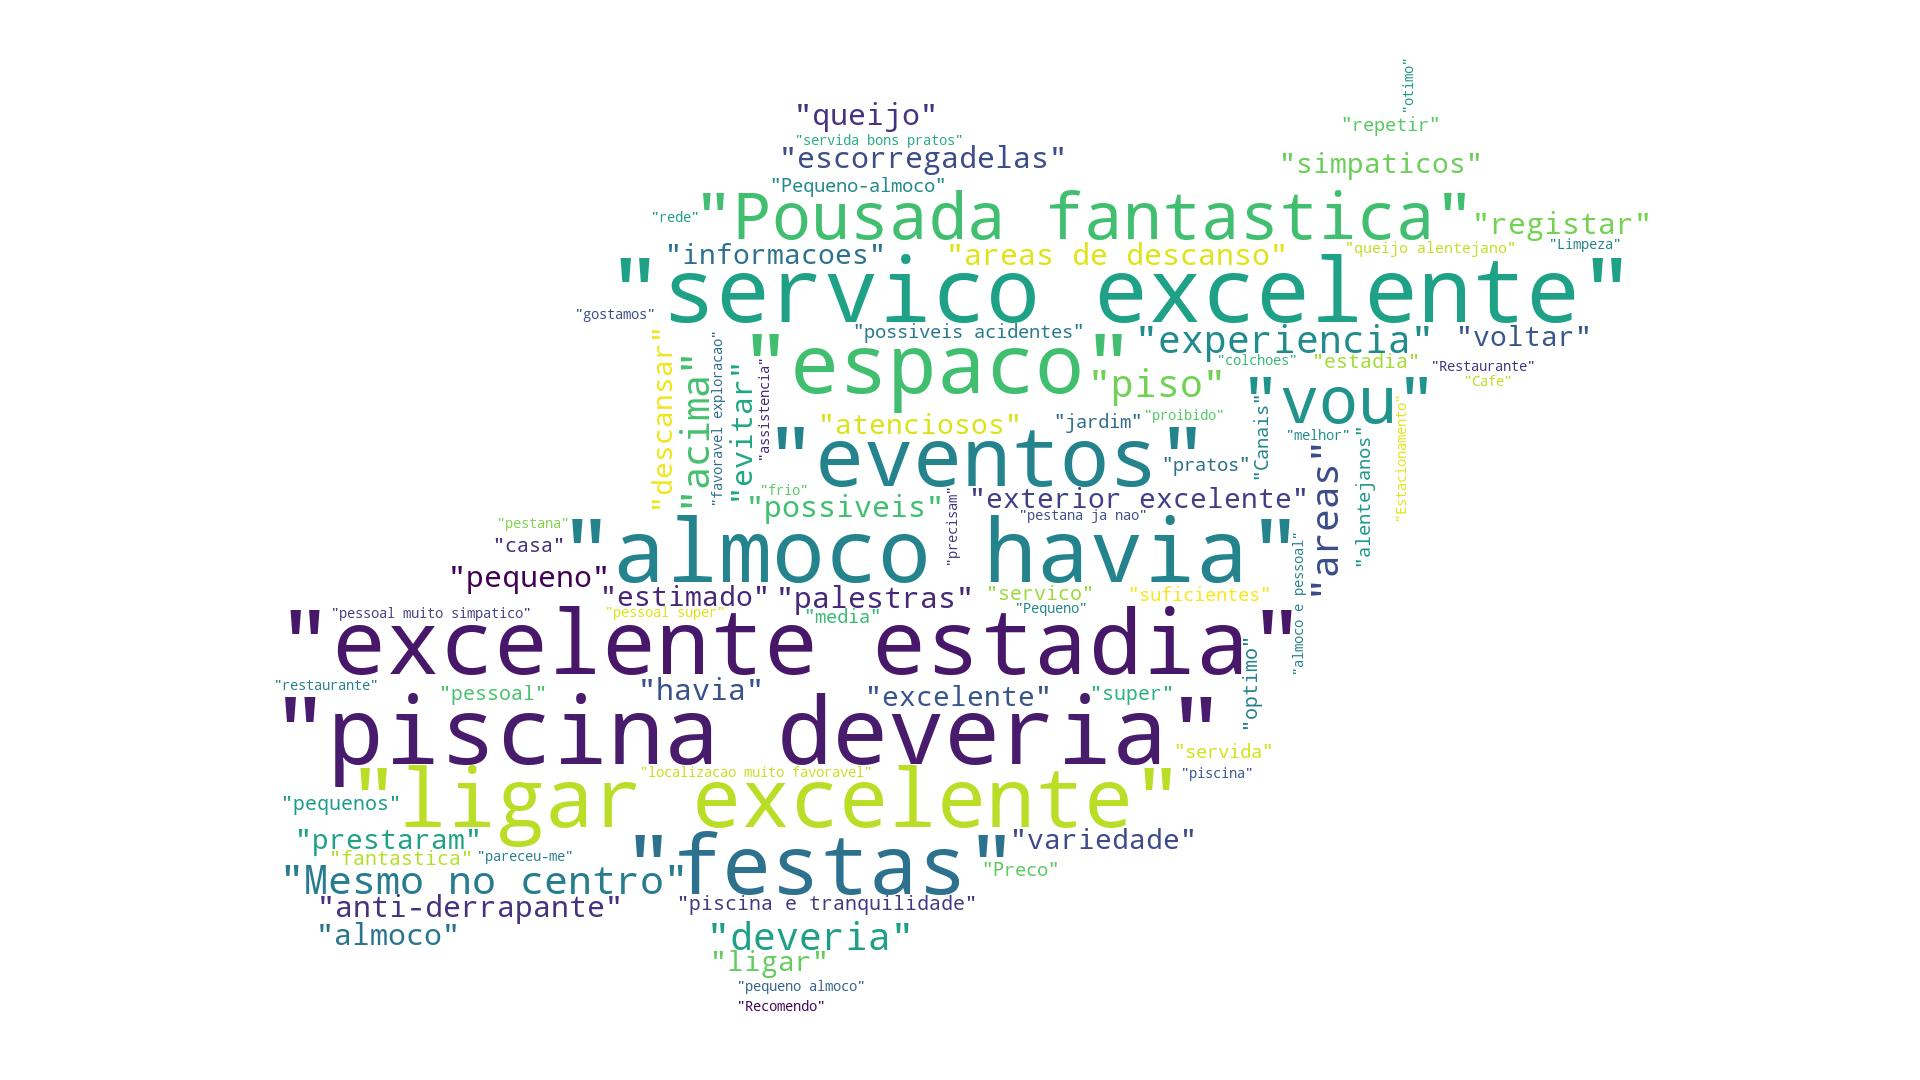
\includegraphics[width=7cm]{figuras/TripAdvisor/Hotels/hotel0_keywordcloud.jpeg}
\caption{Gráfico de palavras-chave e nuvens de palavras-chave contendo as \textit{keywords} mais usadas da plataforma \textit{TripAdvisor} referente à Pousada Convento Beja}
\label{fig:exemplofig}
\end{figure}

\begin{figure}[!htb]
\centering
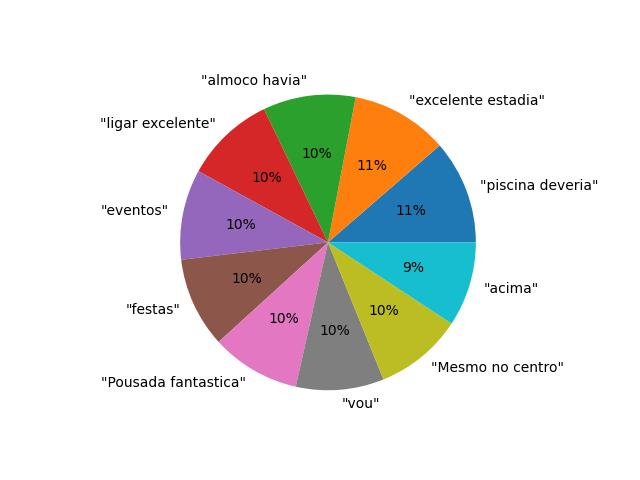
\includegraphics[width=7cm]{figuras/TripAdvisor/Hotels/hotel0_keywords.jpeg}
\caption{Gráfico circular gerado baseando-se nas \textit{keywords} mais usadas da plataforma \textit{TripAdvisor} referente à Pousada Convento Beja}
\label{fig:exemplofig}
\end{figure}

\begin{figure}[!htb]
\centering
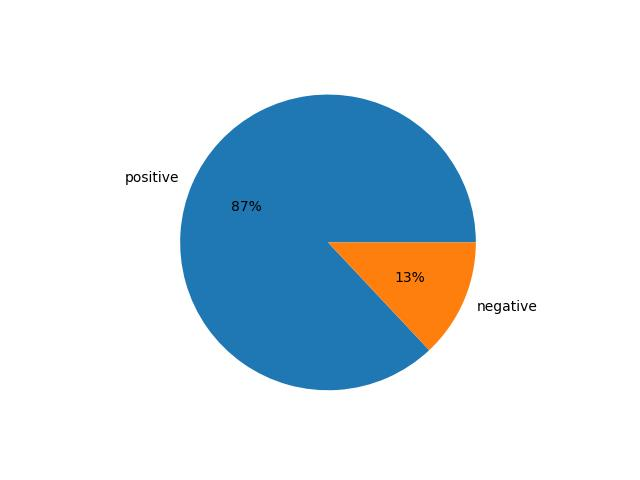
\includegraphics[width=7cm]{figuras/TripAdvisor/Hotels/hotel8_sentiments.jpeg}
\caption{Gráfico circular gerado baseando-se nos \textit{sentiments} mais usados da plataforma \textit{TripAdvisor} referente ao Hotel São Domingos}
\label{fig:exemplofig}
\end{figure}

\begin{figure}[!htb]
\centering
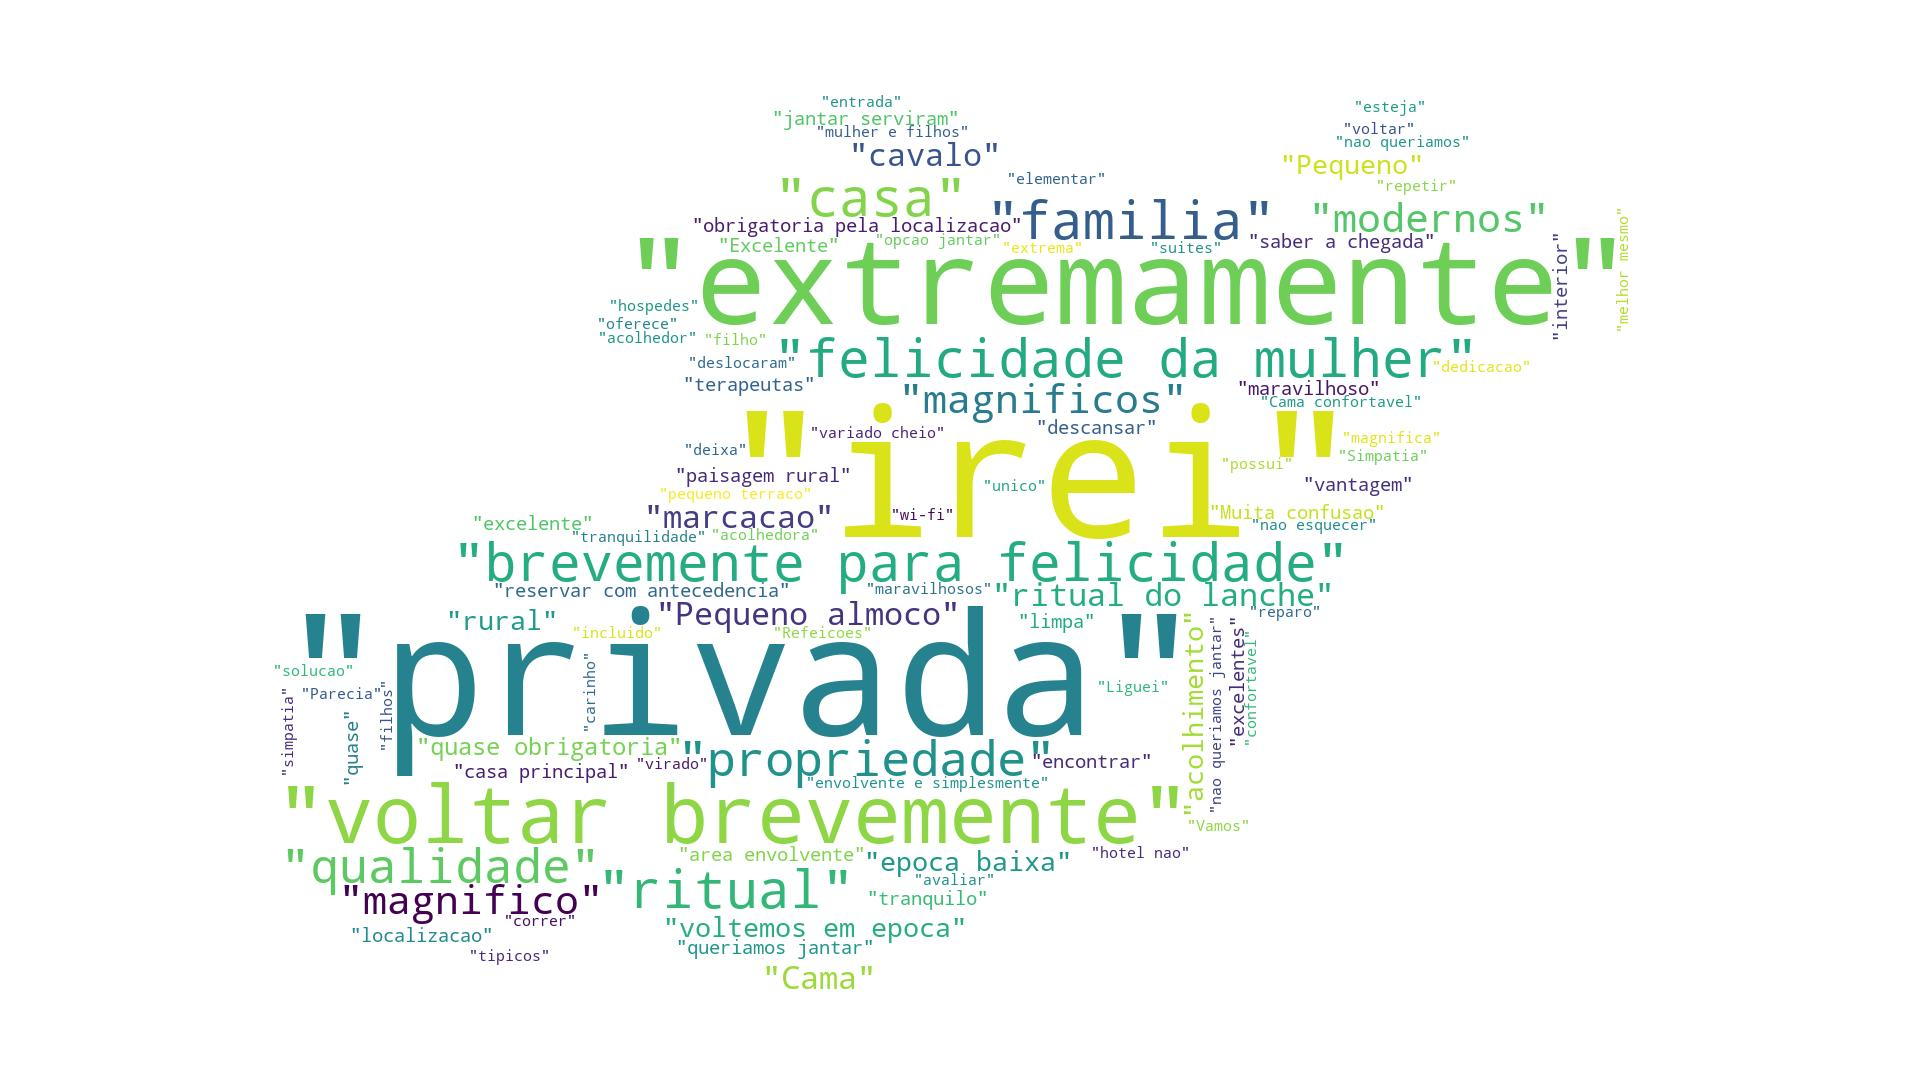
\includegraphics[width=7cm]{figuras/TripAdvisor/Hotels/hotel8_keywordcloud.jpeg}
\caption{Gráfico de palavras-chave e nuvens de palavras-chave contendo as \textit{keywords} mais usadas da plataforma \textit{TripAdvisor} referente ao Hotel São Domingos}
\label{fig:exemplofig}
\end{figure}

\begin{figure}[!htb]
\centering
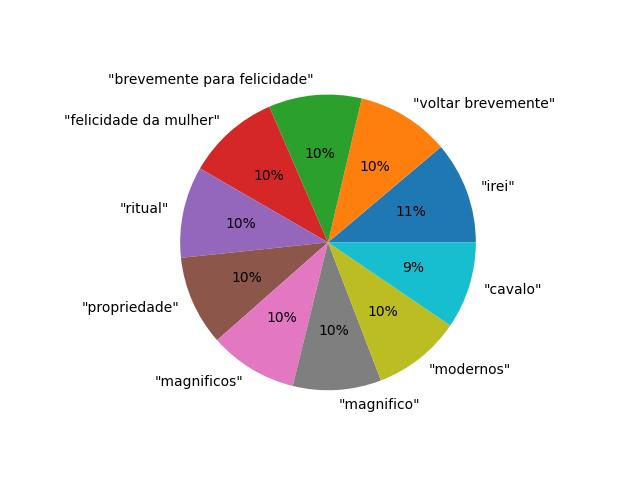
\includegraphics[width=7cm]{figuras/TripAdvisor/Hotels/hotel8_keywords.jpeg}
\caption{Gráfico circular gerado baseando-se nas \textit{keywords} mais usadas da plataforma \textit{TripAdvisor} referente ao Hotel São Domingos}
\label{fig:exemplofig}
\end{figure}

\begin{figure}[!htb]
\centering
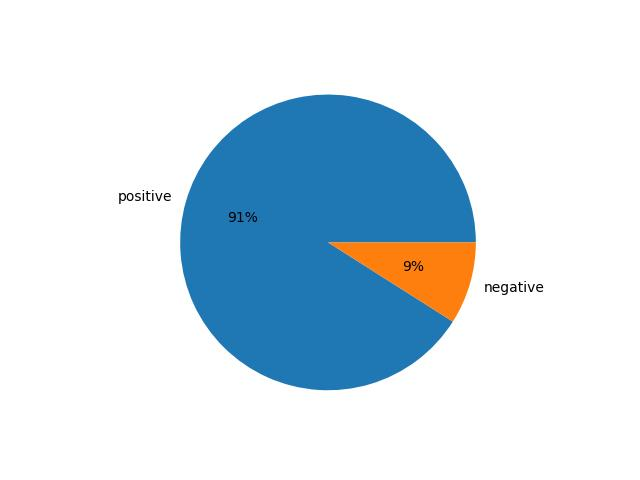
\includegraphics[width=7cm]{figuras/TripAdvisor/Hotels/hotel21_sentiments.jpeg}
\caption{Gráfico circular gerado baseando-se nos \textit{sentiments} mais usados da plataforma \textit{TripAdvisor} referente à Herdade das Barradas da Serra}
\label{fig:exemplofig}
\end{figure}

\begin{figure}[!htb]
\centering
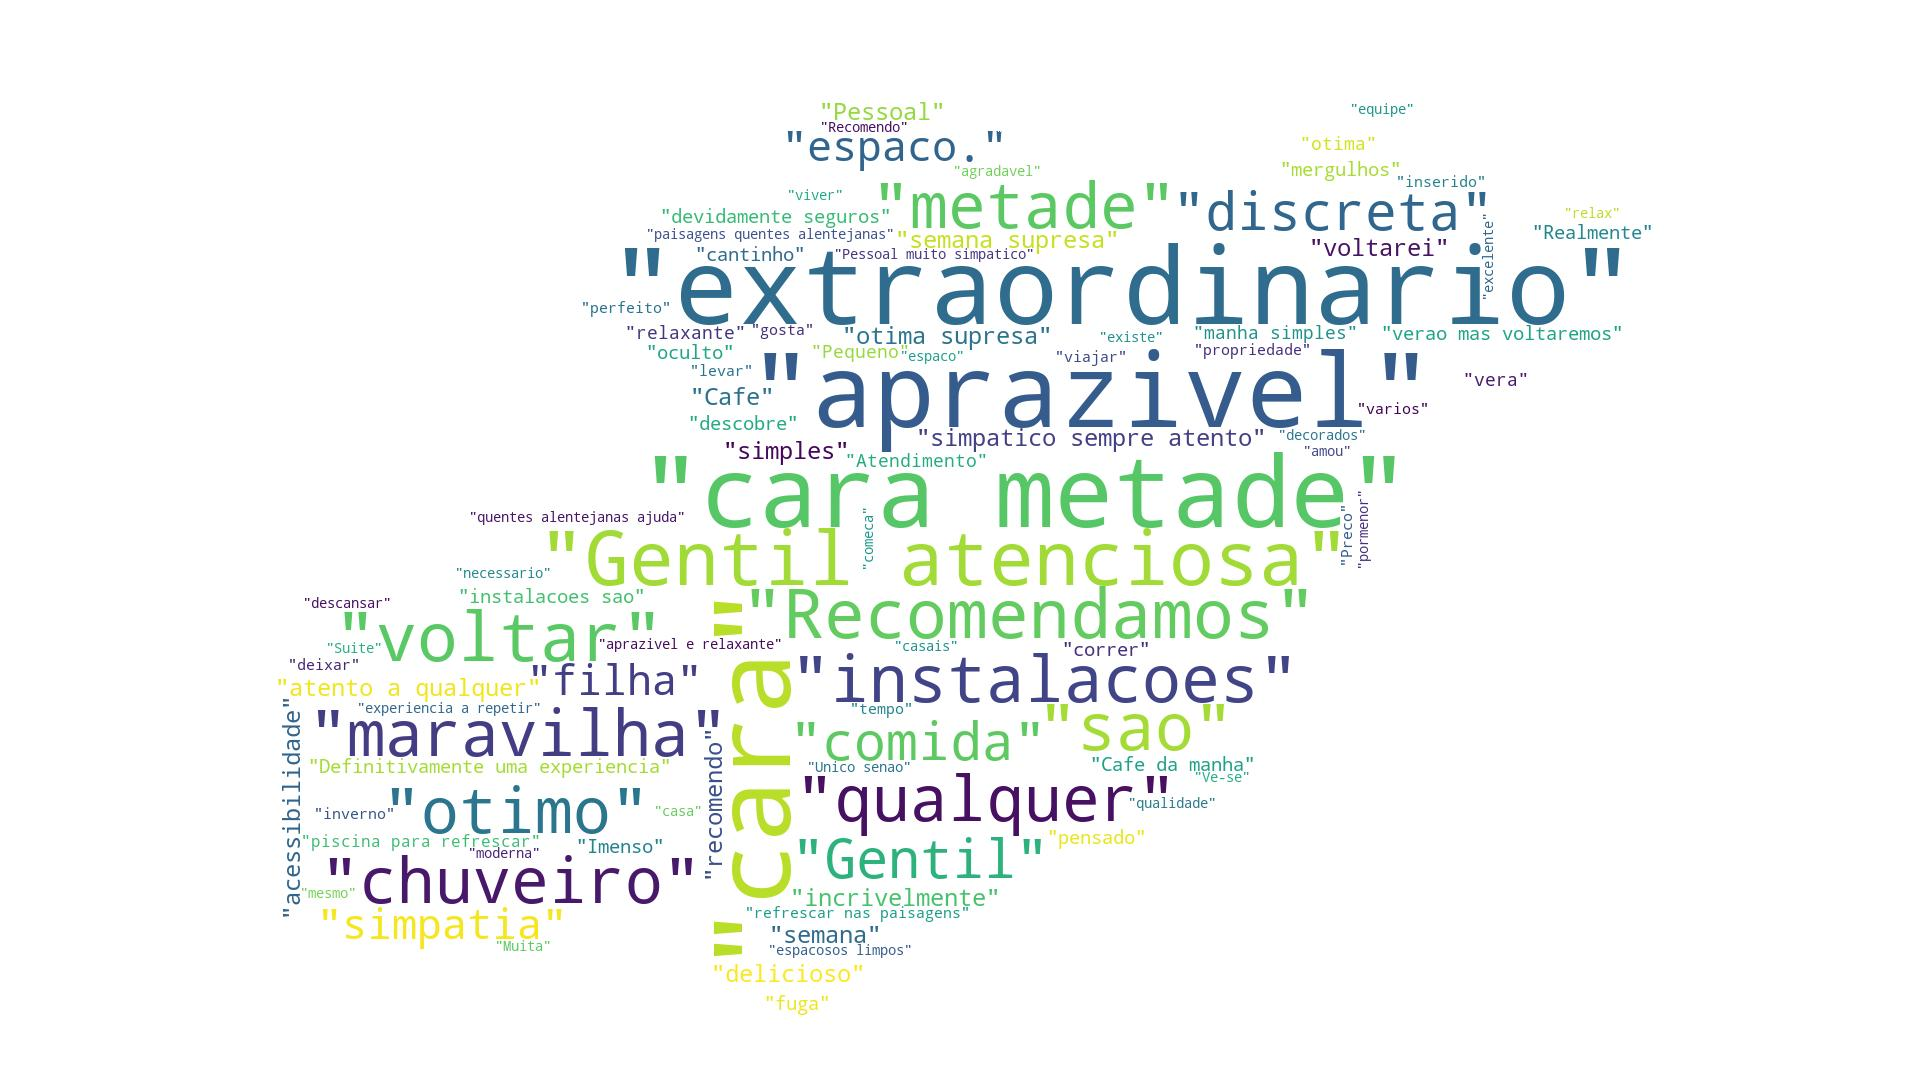
\includegraphics[width=7cm]{figuras/TripAdvisor/Hotels/hotel21_keywordcloud.jpeg}
\caption{Gráfico de palavras-chave e nuvens de palavras-chave contendo as \textit{keywords} mais usadas da plataforma \textit{TripAdvisor} referente à Herdade das Barradas da Serra}
\label{fig:exemplofig}
\end{figure}

\begin{figure}[!htb]
\centering
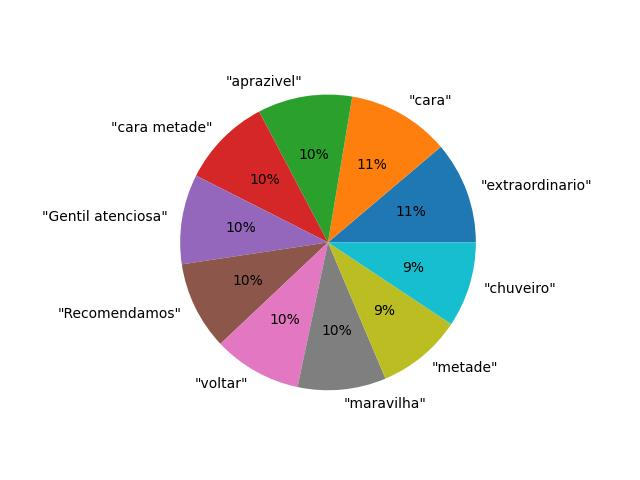
\includegraphics[width=7cm]{figuras/TripAdvisor/Hotels/hotel21_keywords.jpeg}
\caption{Gráfico circular gerado baseando-se nas \textit{keywords} mais usadas da plataforma \textit{TripAdvisor} referente à Herdade das Barradas da Serra}
\label{fig:exemplofig}
\end{figure}

